\documentclass[10pt,letterpaper]{article}

\usepackage[utf8]{inputenc}
\usepackage[T1]{fontenc}
\usepackage{lmodern}
\usepackage{microtype}
\usepackage[top=0.95in,bottom=1.0in,left=1.0in,right=1.0in]{geometry}
\usepackage{amsmath,amssymb}
\usepackage{booktabs}
\usepackage{graphicx}
\usepackage{xcolor}
\usepackage{tcolorbox}
\usepackage{fancyhdr}
\usepackage{enumitem}
\usepackage{natbib}
\usepackage{tikz}
\usetikzlibrary{arrows.meta,positioning,fit,shapes.geometric}
\usepackage[colorlinks=true,linkcolor=blue!50!black,citecolor=blue!50!black,urlcolor=blue!50!black]{hyperref}

\definecolor{sbgray}{RGB}{242,241,238}
\definecolor{sbaccent}{RGB}{35,85,140}
\definecolor{sbgreen}{RGB}{46,125,50}
\definecolor{sbred}{RGB}{198,40,40}
\definecolor{sborange}{RGB}{230,81,0}
\definecolor{sbmuted}{RGB}{95,95,95}

% Page headers and footers matching StoreBench styling
\pagestyle{fancy}
\fancyhf{}
\renewcommand{\headrulewidth}{0pt}
\fancyhead[L]{\small\color{sbmuted}TerrariaBench}
\fancyfoot[C]{\small\thepage}

\fancypagestyle{firstpage}{
  \fancyhf{}
  \renewcommand{\headrulewidth}{0pt}
  \fancyfoot[L]{\small\itshape\color{sbmuted}Pre-print. Copyright 2026 by the author(s).}
  \fancyfoot[C]{\small\thepage}
}

\bibliographystyle{plainnat}

\begin{document}
\thispagestyle{firstpage}

\begin{tcolorbox}[
  colback=sbgray,
  colframe=sbgray,
  arc=6pt,
  boxrule=0pt,
  left=18pt,
  right=18pt,
  top=18pt,
  bottom=16pt
]
{\LARGE\bfseries\raggedright TerrariaBench: A Deterministic Long-Horizon Survival Environment for Evaluating and Training Autonomous Agents\par}
\vspace{10pt}
{\normalsize\bfseries TerrariaBench Contributors\par}
\vspace{2pt}
{\small\color{sbmuted}Junction 2026 --- Break the Agent Track\par}
\vspace{12pt}

\noindent Reinforcement learning (RL) environments are increasingly central to training and evaluating autonomous agents, yet most agentic benchmarks test short, resettable tasks where time advances only when the agent acts and success is a binary terminal check. We introduce \textbf{TerrariaBench}, a deterministic, long-horizon survival and progression benchmark over the Model Context Protocol (MCP) and the containerized Harbor harness, engineered directly on the anchor-calibration and anti-exploit methodology of StoreBench. An agent operates a procedurally seeded Terraria-like world across 4 to 30 alternating 12-hour Day/Night windows through 24 game tools under a strict per-window operation budget, where simulated time advances as a pure function of actions taken so model latency cannot buy extra time. Pass thresholds are calibrated across 70 task-seed cells (14 task lenses $\times$ 5 seeds, including two one-life Hardcore headline tasks) against six scripted anchor policies (\texttt{do-nothing}, \texttt{absentee}, \texttt{blast-list}, \texttt{rule-based}, \texttt{smart-triage}, and \texttt{exploiter}) and four structural gates, while twelve closed reward exploits are regression-tested on every commit. Task prompts disclose the full scoring formula, every checkpoint deadline, and the Hardcore rule while keeping the world seed locked. Across the 24-cell evaluation suite, \texttt{smart-triage} achieves 0.982 (100\% pass); across 8-task standard evaluations, Gemini 4 / 2.5 averages 0.652 (47\% pass, 12 runs; 0.884 over 3 runs on \texttt{eye-of-cthulhu:7}), Nemotron 3.5 VL averages 0.144 (0\% pass, 12 runs), Verda DeepSeek V4.1 Flash scores 0.801 (2 cells, 6 runs), and Verda Kimi K3.1 Pro scores 0.975 (2 cells, 6 runs). Adding the one-life Hardcore rule on \texttt{eye-of-cthulhu-hardcore:7} preserves a stark capability gap against \texttt{smart-triage} (0.985, 0 deaths): across 42 replay-verified transcripts, Kimi K3.1 Pro averages 0.759 (9 runs: 6 wins at 1.00, 3 Window-4 deaths at 0.27--0.28 after its own 25-tile arena overwrote its shelter wall without re-checking), Gemma 4 31B averages 0.403, and DeepSeek V4.1 Flash averages 0.284 on the minimal loop (0.840 via Harbor + OpenCode). Across 23 fatal runs, 14 agents explicitly declared themselves safe immediately before dying. On live 60\,Hz Terraria via our \texttt{tModLoader} bridge, a three-tier vision agent reaches 20\% and 22\% Eye progress across two recorded sessions vs.\ 90\% in symbolic MCP. Finally, closed-loop behavior-cloning (BC) LoRA post-training of \texttt{google/gemma-4-E4B-it} on 652 expert steps raises 8-cell mean composite from 0.249 to 0.720 (deaths $13 \to 3$), and BC-initialized wiki-grounded KL-regularized GRPO ($\beta=0.05$) lifts closed-loop composite from 0.187 to 0.721 (deaths $14 \to 2$, improving 8/8 cells and raising held-out \texttt{cavern-expedition:7} from 0.082 to 0.688 and unseen-seed \texttt{shelter-crunch:17} from 0.174 to 0.843). Beyond game play, these findings highlight both the promise of hierarchical supervisor-plus-reflex architectures (pairing frontier long/short-term planners with low-latency decision layers) and three persistent failure modes in multimodal agents: long-range forethought and plan commitment, smart tactical disengagement (retreating from unwinnable threats rather than fighting), and 2D spatial blind spots after self-modification---yielding concrete lessons for autonomous driving, embodied robotics, and real-world agentic execution.

\vspace{10pt}
{\small\textbf{Public Set \& Code:} \texttt{https://github.com/mairazaini/TerrariaBench} \hfill \textbf{TerrariaBench}}
\end{tcolorbox}

\vspace{10pt}

\section{Introduction}

Reinforcement learning with verifiable rewards has become a primary driver of reasoning and agentic capabilities in large language models (LLMs) \citep{deepseek2025r1,lambert2025tulu3}. As agents transition from single-turn question answering to multi-step operational work \citep{kwa2025measuring,patwardhan2025gdpval}, evaluation suites must measure sustained planning under resource scarcity, hidden deadlines, and compounding consequences. Yet most existing agent benchmarks evaluate bounded tasks in resettable environments \citep{jimenez2024swebench,zhou2024webarena,yao2025taubench}, leaving three structural gaps identified by \citet{raghuvanshi2026storebench}:
\begin{enumerate}[leftmargin=18pt,itemsep=2pt]
  \item \textbf{Asynchronous world progression.} Dusk, hostile spawns, sieges, and boss arrivals occur on the world's clock whether or not the agent is ready. Time must be metered in agent operations rather than wall-clock latency so slow reasoning cannot stall or game the environment.
  \item \textbf{Calibrated cumulative grading.} Long-horizon survival and progression cannot be reduced to an arbitrary binary threshold; partial progress, reliability against hidden deadlines, and attendance must be calibrated against measured scripted baselines.
  \item \textbf{Reward integrity by construction.} Open-ended worlds invite specification gaming---from quitting early to farming placed blocks or resummoning bosses. Rewards must be structurally hardened and continuously tested against an adversarial exploit suite.
\end{enumerate}

We introduce \textbf{TerrariaBench} (Figure~\ref{fig:overview}), a deterministic, long-horizon survival and boss-progression environment that adapts the StoreBench methodology \citep{raghuvanshi2026storebench} to serve as a reproducible proxy for real-world autonomous control: spatial resource management, tech-tree planning, base modification, and real-time tactical survival. Unlike static software or chat sandboxes, real-world domains such as autonomous driving, robotics, and industrial control require a high-level \emph{supervisor} managing long- and short-term strategy to coordinate with a fast \emph{decision and reflex layer} that handles immediate reactions and physical world interaction. The agent interacts exclusively through 24 MCP tools (also exposed via a \texttt{terraria} CLI inside containerized Harbor sandboxes \citep{harbor2026}) over 4 to 30 alternating 12-hour Day/Night windows, while a thin \texttt{tModLoader} socket bridge projects a hierarchical three-tier planner onto live 60\,Hz Terraria. Our contributions are threefold:

\begin{itemize}[leftmargin=18pt,itemsep=3pt]
  \item \textbf{A deterministic, dual-mode long-horizon environment.} TerrariaBench combines spatial exploration, tech-tree dependencies, three perturbation channels (announced, rumored, and silent), full checkpoint/scoring disclosure, and one-life Hardcore risk in a single non-resetting world with zero external runtime dependencies, alongside a live 60\,Hz \texttt{tModLoader} bridge.
  \item \textbf{Calibrated, exploit-hardened evaluation.} Six scripted anchor policies calibrate all 70 task-seed cells (2 Hardcore headline tasks + 8 evaluation tasks + 4 training tasks across 3 reported and 2 held-out seeds) through four quantitative gates, while 12 known reward exploits are structurally closed and pinned by regression tests.
  \item \textbf{Measurable frontier gaps and smaller-model improvement.} On \texttt{eye-of-cthulhu-hardcore} and long-horizon tasks, frontier agents score below the scripted reference due to stale world-state assumptions, budget miscalculation, and cave return failures (even with full scoring and checkpoint transparency), while LoRA post-training on \texttt{google/gemma-4-E4B-it} raises mean composite from 0.249 to 0.720 (BC) and 0.187 to 0.721 (BC+GRPO).
\end{itemize}

\section{Related Work}

\textbf{Agent benchmarks.} Most agentic evaluations measure task completion in static or turn-based settings, including software engineering \citep{jimenez2024swebench}, web and desktop navigation \citep{zhou2024webarena,xie2024osworld}, tool-use dialogues \citep{yao2025taubench}, and workplace simulations \citep{xu2025theagentcompany}. While these benchmarks capture tool syntax and short-horizon reasoning, they reset between tasks and rarely penalize cumulative resource mismanagement or missed intermediate deadlines.

\textbf{Dynamic operational environments.} Gaia2 \citep{froger2026gaia2} introduces asynchronous events but ties timeouts to wall-clock generation latency, whereas Vending-Bench \citep{backlund2025vendingbench} and MerchantBench \citep{shi2026merchantbench} track long-horizon outcomes without anchor-calibrated pass thresholds. StoreBench \citep{raghuvanshi2026storebench} resolves these issues via windowed operation budgets, six scripted calibration anchors, and an audit-close-pin exploit loop. TerrariaBench transfers this exact evaluation architecture from e-commerce to a spatial survival and combat domain.

\textbf{Reward hacking.} Specification gaming and reward tampering remain central failure modes in RL and LLM agents \citep{amodei2016concrete,krakovna2020specification,skalse2022defining,denison2024sycophancy}. Recent benchmarks measure exploit propensity in coding and tool-use agents \citep{zhong2026impossiblebench,zhao2026specbench}. Rather than treating exploits purely as post-hoc diagnostics, TerrariaBench encodes 12 domain-specific exploits into a playable \texttt{exploiter} anchor that must score below every honest anchor on every calibration run.

\begin{figure}[t]
\centering
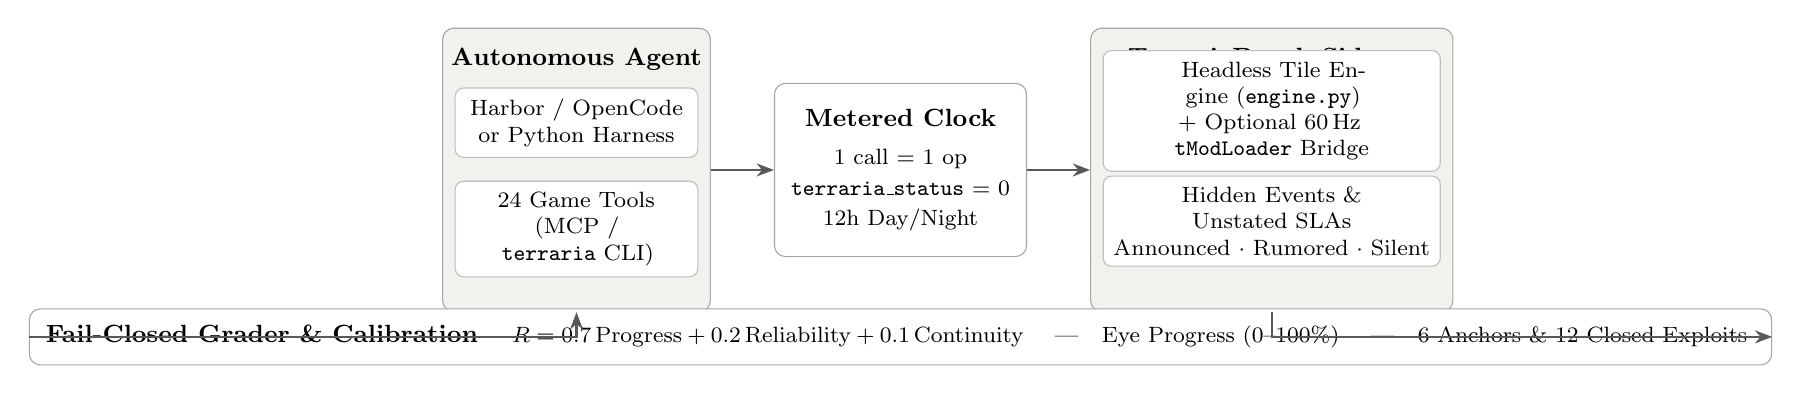
\begin{tikzpicture}[
  box/.style={draw=black!35, rounded corners=4pt, fill=sbgray, align=center, inner sep=6pt, font=\small},
  subbox/.style={draw=black!25, rounded corners=3pt, fill=white, align=center, inner sep=4pt, font=\footnotesize},
  arr/.style={-{Stealth[length=2.2mm]}, thick, color=black!65}
]
  % Agent side
  \node[box, minimum width=3.4cm, minimum height=3.6cm] (agent) {};
  \node[font=\small\bfseries, anchor=north] at ([yshift=-4pt]agent.north) {Autonomous Agent};
  \node[subbox, text width=2.8cm] (harness) at ([yshift=0.6cm]agent.center) {Harbor / OpenCode\\or Python Harness};
  \node[subbox, text width=2.8cm] (tools) at ([yshift=-0.75cm]agent.center) {24 Game Tools\\(MCP / \texttt{terraria} CLI)};

  % MCP / Metered Bridge
  \node[box, right=0.8cm of agent, minimum width=2.4cm, minimum height=2.2cm, fill=white] (mcp) {
    \textbf{Metered Clock}\\[3pt]
    \footnotesize 1 call = 1 op\\
    \footnotesize \texttt{terraria\_status} = 0\\
    \footnotesize 12h Day/Night
  };

  % World side
  \node[box, right=0.8cm of mcp, minimum width=4.6cm, minimum height=3.6cm] (world) {};
  \node[font=\small\bfseries, anchor=north] at ([yshift=-4pt]world.north) {TerrariaBench Sidecar};
  \node[subbox, text width=4.0cm] (sim) at ([yshift=0.75cm]world.center) {Headless Tile Engine (\texttt{engine.py})\\+ Optional 60\,Hz \texttt{tModLoader} Bridge};
  \node[subbox, text width=4.0cm] (dyn) at ([yshift=-0.65cm]world.center) {Hidden Events \& Unstated SLAs\\Announced $\cdot$ Rumored $\cdot$ Silent};

  % Grader bottom
  \node[box, below=0.65cm of mcp, minimum width=11.4cm, fill=white] (grader) {
    \textbf{Fail-Closed Grader \& Calibration} \quad
    \footnotesize $R = 0.7\,\text{Progress} + 0.2\,\text{Reliability} + 0.1\,\text{Continuity}$ \quad|\quad Eye Progress (0--100\%) \quad|\quad 6 Anchors \& 12 Closed Exploits
  };

  \draw[arr] (agent.east) -- (mcp.west);
  \draw[arr] (mcp.east) -- (world.west);
  \draw[arr] (world.south) |- (grader.east);
  \draw[arr] (grader.west) -| (agent.south);
\end{tikzpicture}
\caption{TerrariaBench architecture. A harness-agnostic agent interacts with an isolated game sidecar exclusively through 24 MCP tools (or the \texttt{terraria} CLI). Each action spends one operation from the window budget; when operations exhaust or \texttt{end\_window} is called, the remainder of the 12-hour window plays out. At episode end, a fail-closed verifier settles unattended windows and grades the SHA-256-sealed ledger.}
\label{fig:overview}
\end{figure}

\section{The TerrariaBench Environment}

\subsection{A World with Deterministic Provenance}
TerrariaBench simulates a 2D tile-based survival world with surface forest, underground stone and ore veins (copper, iron, gold), cavern Life Crystals, corruption spread, and an underworld layer. Each world is keyed by an integer seed and driven by purpose-keyed SHA-256 random streams (\texttt{provenance.stream}), ensuring that unrelated inspection calls cannot shift future loot, enemy spawns, or boss behavior. Replaying any recorded action sequence reproduces the terminal state and SHA-256-sealed ledger byte for byte.

\subsection{Hidden Dynamics and Three Perturbation Channels}
World hazards and obligations evolve across alternating 12-hour Day and Night windows (27,000 simulated ticks at 60\,Hz per window). Following \citet{raghuvanshi2026storebench}, events perturb the world through three channels:
\begin{itemize}[leftmargin=18pt,itemsep=2pt]
  \item \textbf{Announced:} explicit alerts with advance lead time (e.g., Goblin Siege announced at window 6 before arriving at window 9; Blood Moon announced at window 5 before window 6).
  \item \textbf{Rumored:} vague environmental cues without exact timing or numbers (e.g., \texttt{eye\_spawn}, \texttt{cave\_chill}).
  \item \textbf{Silent:} unannounced hazards visible only through telemetry or combat outcomes (e.g., nocturnal spawn spikes, hidden cavern traps, corruption spread, and Eye of Cthulhu Phase 2 enrage).
\end{itemize}
To prevent seed overfitting, evaluation runs set \texttt{redact\_seed=True}, replacing the world seed in the status header with \texttt{World: locked}. To eliminate artificial specification surprises, every task prompt (\texttt{Task.prompt}) explicitly states the full composite scoring rule, every SLA checkpoint deadline, and (for Hardcore variants) the one-life termination rule and main causes of death; a test in \texttt{tests/test\_evaluation.py} fails if any graded checkpoint is omitted from the prompt.

\subsection{Tasks as Lenses}
TerrariaBench defines 14 task lenses over the shared seeded world: 2 one-life Hardcore variants (\texttt{first-night-hardcore}, \texttt{eye-of-cthulhu-hardcore}), 8 evaluation tasks (\texttt{EVAL\_TASKS}), and 4 disjoint shorter-horizon training tasks (\texttt{TRAIN\_TASKS}), summarized in Appendix~\ref{app:tasks}. Each lens configures the horizon $W \in [4, 30]$ windows, per-window operation budget $B \in [11, 20]$, starting kit, event script, and stated SLA deadlines (e.g., enclosed shelter by dusk, iron-tier gear by window 8, multi-tier boss arena by window 10, Eye of Cthulhu defeat by window 14). Three world seeds (7, 11, 13) form the reported evaluation grid, while seeds 17 and 23 serve as held-out calibration and generalization seeds (70 calibrated cells total).

\subsection{Tool Surface and Metered Time}
The agent acts through 24 tools spanning five families (Appendix~\ref{app:tools}): Status \& Time (2), Observation \& Spatial Inspection (5), Gathering, Mining \& Navigation (5), Crafting, Building \& Blueprints (6), and Combat \& Boss Control (6). Every tool reply prepends a one-line state header:
\begin{center}
\small\texttt{[World: locked | Win: ... | Ops: ... | HP: ... | Mana: ... | Def: ... | NetProg: ... | TechTier: ... | Threat: ...]}
\end{center}
Every tool call costs 1 operation except \texttt{terraria\_status} (0 operations). Operations do not roll over across windows. Thus, reading the viewport (\texttt{observe\_viewport}) or scanning ores (\texttt{scan\_biome\_and\_ores}) competes directly with gathering, crafting, and combat for the same scarce budget. When operations reach zero or the agent calls \texttt{end\_window}, the remaining ticks of the 12-hour window resolve with the player standing at its current position: an unsheltered agent at night takes hostile damage, and dying forfeits 50\% of raw materials plus operations in the following window.

\subsection{Live \texttt{tModLoader} Bridge and Real-Game Recording}
Beyond the fast headless simulator, TerrariaBench includes a C\# \texttt{tModLoader} mod (\texttt{mod/TerrariaRLBridge/}) that exports 60\,Hz Terraria state and referee kill/death telemetry alongside skill macros (\texttt{Skills.cs}) executed via OS keyboard and mouse control (\texttt{real\_game.py}, \texttt{live\_play.py}). A three-tier Gemini vision-and-strategy loop runs against live Terraria pixels, while \texttt{terraria\_bench/real\_eval.py} scores committed recordings offline across 13 Eye-of-Cthulhu progression stages with tamper-evident referee consistency checks.

\section{Grader Design}

\subsection{Composite Score and Eye Progress}
At episode end, the verifier calls \texttt{/finalize} on the isolated game sidecar, which settles any unplayed windows with the player idle and computes the StoreBench-adapted composite score $R \in [0, 1]$:
\begin{equation}
  R = \underbrace{0.7\,\mathrm{clip}_{[0,1]}\!\left(\frac{\Delta\mathrm{net} - z}{s}\right)}_{\text{progress (business)}}
    + \underbrace{0.2\,\frac{1}{2}\!\left(\text{survival\_rate} + \text{sla\_rate}\right)}_{\text{reliability}}
    + \underbrace{0.1\,\left(\frac{\text{windows\_attended}}{\text{windows\_in\_task}}\right)\mathrm{clip}_{[0,1]}\!\left(\frac{\text{business}}{0.10}\right)}_{\text{continuity}},
  \label{eq:composite}
\end{equation}
where $\Delta\mathrm{net}$ is the growth in Net Progression Value (crafted gear, placed structures, cavern depth, events survived, and boss damage, with raw materials discounted by $\rho = 0.15$ to prevent hoarding), and $z$ and $s$ are the sealed absentee baseline and anchor range for that task-seed cell. Crucially, continuity is gated on normalized progress ($\text{business} / 0.10$) and divides by the full task window count, ensuring that both quitting early and attending every window while doing nothing score $0.000$. An unclipped dense channel ($\text{DENSE\_CLIP} = [-2.0, 1.0]$) is also exported for RL training (Appendix~\ref{app:dense}).

Alongside the composite score, every simulator grade and live \texttt{tModLoader} session reports \textbf{Eye progress} (0--100\%, \texttt{compute\_eye\_progress}), a monotonic high-water-mark metric toward defeating the Eye of Cthulhu: Health (+10\% up to +80 max HP), Armor (+10\% up to 8 defense), Tech-tree milestones (+35\%), Boss damage (+5\% on first hit plus up to +20\% by lowest Eye HP reached), and Boss kill (exact 100\%; capped at 80\% without a kill).

\subsection{Anchor Calibration and Structural Gates}
For every task-seed cell (70 cells across all 14 tasks and 5 seeds), TerrariaBench runs six scripted anchor policies through the exact tool surface: \texttt{do-nothing}, \texttt{absentee} (calls \texttt{end\_window} every window), \texttt{blast-list} (spends ops on naive gathering/inspection), \texttt{rule-based} (checklist progression), \texttt{smart-triage} (prioritized survival, SLA timing, paced housing safety, and combat), and \texttt{exploiter} (replays the playable reward-exploit catalogue). The pass threshold is placed between the top two honest anchors and must pass four automated calibration gates (\texttt{tests/test\_calibration\_gates.py}):
\begin{enumerate}[leftmargin=18pt,itemsep=2pt]
  \item \textbf{Ordering:} both judgment anchors (\texttt{rule-based}, \texttt{smart-triage}) must strictly outscore \texttt{blast-list}, \texttt{absentee}, and \texttt{do-nothing}.
  \item \textbf{Judgment gap:} the top honest anchor must exceed \texttt{blast-list} by at least 0.15.
  \item \textbf{Flap margin:} the pass threshold must clear adjacent anchors by at least 0.02.
  \item \textbf{Exploit suppression:} \texttt{exploiter} must score below 0.05 and below every honest trading anchor.
\end{enumerate}
All 70 cells in \texttt{artifacts/calibration.json} pass all four gates (\texttt{all\_gates\_passed = True}; Figure~\ref{fig:ladder}).

\begin{figure}[t]
\centering
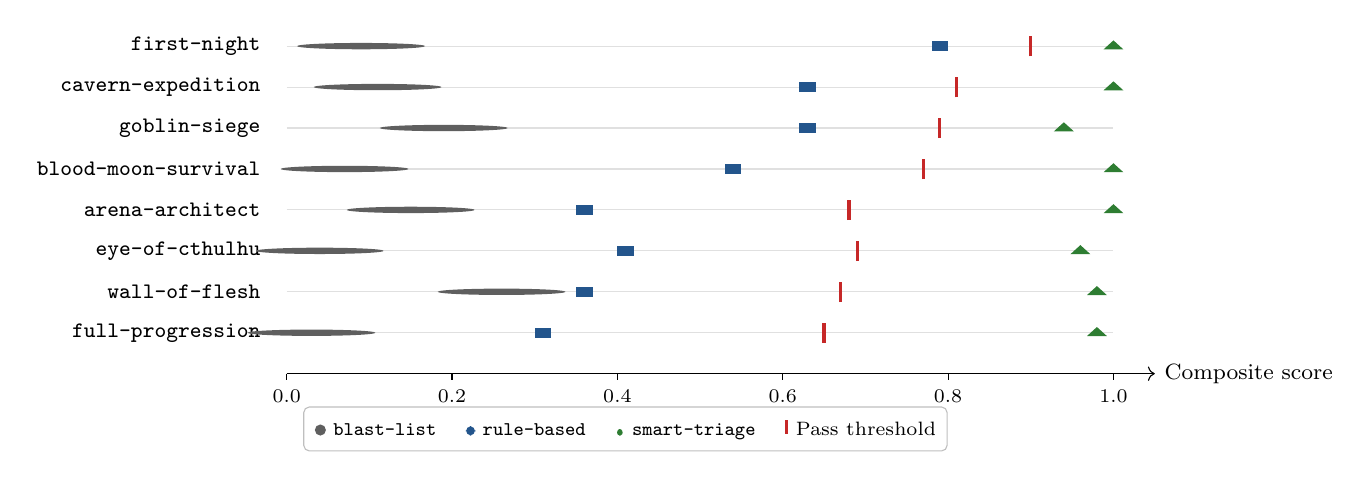
\begin{tikzpicture}[xscale=10.5, yscale=0.52]
  % Axes
  \draw[->] (0,0) -- (1.05,0) node[right,font=\footnotesize] {Composite score};
  \foreach \x in {0.0,0.2,0.4,0.6,0.8,1.0} {
    \draw (\x,0) -- (\x,-0.15) node[below,font=\scriptsize] {\x};
  }
  % Tasks from top to bottom (y=8 down to 1)
  \foreach \y/\name/\bl/\rb/\st/\th in {
    8/first-night/0.09/0.79/1.00/0.90,
    7/cavern-expedition/0.11/0.63/1.00/0.81,
    6/goblin-siege/0.19/0.63/0.94/0.79,
    5/blood-moon-survival/0.07/0.54/1.00/0.77,
    4/arena-architect/0.15/0.36/1.00/0.68,
    3/eye-of-cthulhu/0.04/0.41/0.96/0.69,
    2/wall-of-flesh/0.26/0.36/0.98/0.67,
    1/full-progression/0.03/0.31/0.98/0.65
  } {
    \draw[black!12] (0,\y) -- (1.0,\y);
    \node[left,font=\footnotesize] at (-0.02,\y) {\texttt{\name}};
    \fill[sbmuted] (\bl,\y) circle (2.2pt);
    \fill[sbaccent] (\rb-0.01,\y-0.12) rectangle (\rb+0.01,\y+0.12);
    \fill[sbgreen] (\st,\y+0.14) -- (\st-0.012,\y-0.08) -- (\st+0.012,\y-0.08) -- cycle;
    \draw[sbred, very thick] (\th,\y-0.25) -- (\th,\y+0.25);
  }
  % Legend
  \node[draw=black!25,fill=white,rounded corners=2pt,anchor=north west,font=\scriptsize,inner sep=4pt] at (0.02, -0.8) {
    \tikz{\fill[sbmuted] (0,0) circle (2pt);} \texttt{blast-list} \quad
    \tikz{\fill[sbaccent] (0,0) rectangle (0.12,0.12);} \texttt{rule-based} \quad
    \tikz{\fill[sbgreen] (0,0.12) -- (-0.06,0) -- (0.06,0) -- cycle;} \texttt{smart-triage} \quad
    \tikz{\draw[sbred,very thick] (0,0) -- (0,0.18);} Pass threshold
  };
\end{tikzpicture}
\vspace{16pt}
\caption{Mean anchor ladder across seeds $\{7, 11, 13\}$ for the eight evaluation tasks. On every cell, \texttt{do-nothing}, \texttt{absentee}, and \texttt{exploiter} sit at $0.00$, while the calibrated threshold cleanly separates \texttt{rule-based} from \texttt{smart-triage}. Full per-seed values are in Appendix~\ref{app:calibration}.}
\label{fig:ladder}
\end{figure}

\subsection{Reward Integrity and Fail-Closed Provenance}
Twelve reward exploits are catalogued in \texttt{terraria\_bench.grader.EXPLOITS} (Appendix~\ref{app:exploits}), including \texttt{continuity\_for\_quitters}, \texttt{attendance\_farming}, \texttt{dirt\_box\_camping}, \texttt{place\_break\_farming}, \texttt{slime\_grinding}, \texttt{boss\_resummon\_scumming}, \texttt{craft\_trash\_cycling}, \texttt{suicide\_respawn\_teleport}, \texttt{last\_window\_dumping}, \texttt{partial\_enclosure\_spoofing}, \texttt{chest\_duplicate\_looting}, and \texttt{healing\_potion\_stalling}. Each is structurally closed in the engine/grader and pinned by an adversarial test in \texttt{tests/test\_reward\_exploits.py}.

In Harbor evaluations, the simulator, sealed calibration, and ledger reside in an isolated \texttt{game} sidecar container unreachable from the agent's filesystem; only \texttt{POST /finalize} with a task-specific \texttt{X-Verifier-Token} triggers grading. Missing or tampered artifacts grade to $0.0$.

\section{Experimental Setup}

\textbf{Protocol.} We evaluate all six scripted anchors deterministically across the 24 reported standard evaluation cells (8 evaluation tasks $\times$ seeds $\{7, 11, 13\}$) and both one-life Hardcore headline tasks (\texttt{first-night-hardcore}, \texttt{eye-of-cthulhu-hardcore}). For model evaluation, we combine (i) sealed runs on the 8-task standard grid (\texttt{EVAL\_RESULTS.md}, covering Gemini 4 / 2.5, Nemotron 3.5 VL, Verda Kimi K3.1 Pro, Verda DeepSeek V4.1 Flash, Gemma 4 E4B Base, and a human operator), (ii) 42 single-call minimal-loop transcripts (\texttt{evaluation/run\_model.py}, replayed offline by \texttt{evaluation/judge.py} across Hardcore and normal tasks for Kimi K3.1 Pro, DeepSeek V4.1 Flash, and Gemma 4 31B), (iii) Harbor + OpenCode over MCP trials (\texttt{results/harbor\_agent/}), and (iv) two live 60\,Hz real-Terraria recordings scored offline against referee telemetry (\texttt{terraria\_bench/real\_eval.py}). All model numbers derive strictly from sealed ledgers and engine replay.

\textbf{Post-training setup.} To test whether smaller open models can improve from environment experience, we extract 652 turn-by-turn expert trajectories from \texttt{smart-triage} across the four disjoint training tasks (\texttt{woodland-scramble}, \texttt{ore-rush}, \texttt{slime-rain}, \texttt{shelter-crunch}; seeds 7, 11, 13), keeping only episodes grading $\ge 0.95$ with zero deaths. We fine-tune \texttt{google/gemma-4-E4B-it} with a rank-32 LoRA \citep{hu2022lora} via behavior cloning (\texttt{post\_training/modal\_grpo\_gemma.py}) and evaluate base vs.\ tuned checkpoints with identical prompts and greedy decoding over eight cells spanning seen training cells, unseen seed 17, and unseen evaluation tasks (\texttt{first-night:7}, \texttt{cavern-expedition:7}).

\section{Evaluation Results}

\subsection{Standard Grid, Hardcore Gap, and 42-Run Autopsy}
Table~\ref{tab:leaderboard} reports the reproducible standard leaderboard from \texttt{reporting/generate\_report.py}. Across the full 24-cell evaluation suite, \texttt{smart-triage} achieves a mean composite of \textbf{0.982} (100\% pass rate, 57\% Eye progress), \texttt{rule-based} reaches \textbf{0.505} (0\% pass rate), and \texttt{blast-list} scores \textbf{0.116}. All three non-progress baselines---\texttt{do-nothing}, \texttt{absentee}, and \texttt{exploiter}---score \textbf{0.000}. Notice that repeat runs of one cell are averaged into that cell first so repeated headline episodes do not re-weight a model's row. Across 10 evaluated cells (12 sealed runs), Gemini 4 / 2.5 averages \textbf{0.652} (47\% pass rate; averaging \textbf{0.884} over three uncapped \texttt{eye-of-cthulhu:7} runs: 0.971, 0.682, 1.000), while Nemotron 3.5 VL averages \textbf{0.144} across 10 cells (12 runs, 0\% pass; \textbf{0.108} on \texttt{eye-of-cthulhu:7}). On the 2-cell seed-7 replay subset (\texttt{first-night:7}, \texttt{eye-of-cthulhu:7}), Verda DeepSeek V4.1 Flash averages \textbf{0.801} (50\% pass, 6 runs) and Verda Kimi K3.1 Pro averages \textbf{0.975} (67\% pass, 6 runs).

\begin{table}[t]
\centering
\caption{TerrariaBench standard simulator leaderboard (\texttt{reporting/generate\_report.py}). Scripted anchors span all 24 cells (8 eval tasks $\times$ seeds 7, 11, 13). Model and human rows average cells first (repeating \texttt{eye-of-cthulhu:7} does not re-weight the mean) over all sealed ledgers in \texttt{artifacts/runs/} and verified normal-task transcripts in \texttt{results/runs/}.}
\label{tab:leaderboard}
\begin{tabular}{llrrrrr}
\toprule
Policy / Model & Status & Cells & Runs & Composite & Pass rate & Eye progress \\
\midrule
\textit{smart-triage} & anchor & 24 & 24 & \textbf{0.982} & \textbf{100\%} & \textbf{57\%} \\
\textit{rule-based} & anchor & 24 & 24 & 0.505 & 0\% & 32\% \\
\textit{blast-list} & anchor & 24 & 24 & 0.116 & 0\% & 4\% \\
\textit{absentee} (stop-early) & anchor & 24 & 24 & 0.000 & 0\% & 0\% \\
\textit{do-nothing} & anchor & 24 & 24 & 0.000 & 0\% & 0\% \\
\textit{exploiter} & anchor & 24 & 24 & 0.000 & 0\% & 0\% \\
\midrule
Verda Kimi K3.1 Pro & evaluated & 2 & 6 & 0.975 & 67\% & 70\% \\
Verda DeepSeek V4.1 Flash & evaluated & 2 & 6 & 0.801 & 50\% & 66\% \\
Gemini 4 / 2.5 & evaluated & 10 & 12 & 0.652 & 47\% & 45\% \\
Human experts & evaluated & 1 & 1 & 0.489 & 0\% & 19\% \\
Nemotron 3.5 VL & evaluated & 10 & 12 & 0.144 & 0\% & 15\% \\
Gemma 4 E4B Base & evaluated & 4 & 4 & 0.046 & 0\% & 12\% \\
\bottomrule
\end{tabular}
\end{table}

\textbf{Why Hardcore exposes the true capability gap (42-run autopsy).} When scoring rules and checkpoints are disclosed on normal soft-death tasks, strong models match or exceed the scripted reference on single runs (\texttt{eye-of-cthulhu:7}: Kimi K3.1 Pro \textbf{0.989}, DeepSeek V4.1 Flash \textbf{0.908} vs.\ reference \textbf{0.950}), yet frequently die during preparation (Kimi dies once in 5 of 6 normal-task runs; DeepSeek dies 5 times in one run and still scores 0.758). Enabling the one-life Hardcore rule (Table~\ref{tab:hardcore}) separates agents cleanly even when all rules are disclosed: on \texttt{eye-of-cthulhu-hardcore:7}, \texttt{smart-triage} scores \textbf{0.985} (0 deaths), whereas DeepSeek averages \textbf{0.284} (3 runs), Gemma 4 31B averages \textbf{0.403} (3 runs), and Kimi K3.1 Pro averages \textbf{0.759} across 9 runs---scoring a perfect \textbf{1.000} on 6/9 runs yet dying in Window 4 at \textbf{0.267--0.283} on 3/9 runs. Over Harbor + OpenCode via MCP, scaffolding lifts DeepSeek V4.1 Flash on \texttt{terraria-eye-of-cthulhu-hardcore} to \textbf{0.840} mean across 3 trials (0.523, 0.996, 1.000), and Kimi scores \textbf{1.000} on the 1 trial that started.

\begin{table}[t]
\centering
\caption{Hardcore vs.\ normal headline results on seed 7 under full checkpoint and scoring disclosure (\texttt{evaluation/run\_model.py}, replayed in \texttt{RESULTS.md}, 42 transcripts). Number of runs in parentheses.}
\label{tab:hardcore}
\begin{tabular}{lcccc}
\toprule
Player & \texttt{first-night-hc} & \texttt{eye-cthulhu-hc} & \texttt{first-night} & \texttt{eye-cthulhu} \\
\midrule
\textbf{Reference (\textit{smart-triage})} & \textbf{1.000} & \textbf{0.985} & \textbf{1.000} & \textbf{0.950} \\
Pass threshold & 0.860 & 0.659 & 0.950 & 0.696 \\
\midrule
Kimi K3.1 Pro & 0.827 (3) & 0.759 (9) & 0.961 (3) & 0.989 (3) \\
Gemma 4 31B & 0.648 (3) & 0.403 (3) & 0.716 (3) & 0.711 (3) \\
DeepSeek V4.1 Flash & 0.660 (3) & 0.284 (3) & 0.695 (3) & 0.908 (3) \\
Do nothing & 0.000 & 0.000 & 0.000 & 0.000 \\
\bottomrule
\end{tabular}
\end{table}

Replaying all 42 transcripts reveals \textbf{23 runs with at least one death} across three failure mechanisms (\texttt{FAILURE\_ANALYSIS.md}):
(1) \emph{Trusting stale world state} (\textbf{9/23} first deaths, including all 3 of Kimi's Hardcore deaths): building a 25-tile boss arena beside home breaks the shelter wall; 7/9 Kimi runs caused this collision---the 4 that spent one operation re-checking and repaired scored \textbf{1.000}, whereas the 3 that failed to verify or dismissed an \texttt{invalid} warning died in their sleep (\textbf{0.27--0.28}).
(2) \emph{Unwinnable boss clock} (\textbf{7/23} deaths): summoning the 2,800-HP Eye late in a window when observable per-burst damage makes finishing before window close impossible.
(3) \emph{Zero cave return margin} (\textbf{7/23} deaths): exhausting operations underground instead of tracking \texttt{navigate\_to} return distance. Across \textbf{14 of the 23 fatal runs}, the model's stated reason for its final action explicitly claimed it was safe immediately before dying.

\textbf{Sim-to-Real 60\,Hz Terraria gap.} In symbolic MCP simulation, the Gemini two-tier agent averages \textbf{90\%} Eye progress (killing the Eye in 3 of 4 runs). Projecting into live 60\,Hz \texttt{tModLoader} Terraria via pixels, keyboard, and mouse (\texttt{real\_eval.py}, Table~\ref{tab:live60hz}), two 300-frame live sessions with the four-role hierarchical stack (\texttt{gemini-4-carbon} supervisor, \texttt{gemini-4-hydrogen} short-term/vision, \texttt{gemini-decision-1} reflex) reach \textbf{20\%} Eye progress (\texttt{real\_terraria\_run1.json}: 4/13 stages, 2 deaths) and \textbf{22.3\%} Eye progress (\texttt{real\_terraria\_run2.json}: 6/13 stages adding furnace smelting and armor equipping, 0 deaths), both stalling at \texttt{ammunition\_ready} with consistent offline referee telemetry. Median latencies explain why a fast decision tier is essential: the frontier supervisor takes 32.8--46.2\,s per strategic update, whereas the decision/reflex tier responds in 0.57--0.78\,s.

\begin{table}[t]
\centering
\caption{Live 60\,Hz \texttt{tModLoader} Terraria agent performance (\texttt{artifacts/runs/real\_terraria/summary.json}) vs.\ symbolic MCP simulation. Both live sessions run 300 frames with \texttt{gemini-4-carbon} (supervisor), \texttt{gemini-4-hydrogen} (short-term \& vision), and \texttt{gemini-decision-1} (reflex).}
\label{tab:live60hz}
\begin{tabular}{lccccc}
\toprule
Session & Stages & Eye Prog. & Deaths & Stall Stage & Med.\ Latency (Sup.\ / Dec.) \\
\midrule
Symbolic MCP (Gemini, 4 runs) & --- & \textbf{90\%} (3/4 kills) & --- & --- & --- \\
Live 60\,Hz Run 1 (\texttt{real\_terraria\_run1}) & 4/13 & 20.0\% & 2 & \texttt{ammunition\_ready} & 32.81\,s / 0.57\,s \\
Live 60\,Hz Run 2 (\texttt{real\_terraria\_run2}) & 6/13 & 22.3\% & 0 & \texttt{ammunition\_ready} & 46.24\,s / 0.78\,s \\
\bottomrule
\end{tabular}
\end{table}

\subsection{Three Failure Areas}
Table~\ref{tab:areas} groups the 8-task standard evaluation suite into three capability axes (\texttt{EVAL\_RESULTS.md}):
\begin{table}[t]
\centering
\caption{Mean composite score by failure area across scripted anchors (all 3 reported seeds) and evaluated cells (\texttt{EVAL\_RESULTS.md}).}
\label{tab:areas}
\begin{tabular}{llcccc}
\toprule
Failure area & Tasks & \textit{smart-triage} & \textit{rule-based} & Gemini 4 / 2.5 & Nemotron 3.5 VL \\
\midrule
Long-range strategy planning & \texttt{goblin-siege}, \texttt{eye-of-cthulhu}, & \textbf{0.964} & 0.429 & 0.813 & 0.146 \\
 & \texttt{wall-of-flesh}, \texttt{full-progression} & & & & \\
Short-range strategy \& execution & \texttt{first-night}, \texttt{blood-moon-survival} & \textbf{1.000} & 0.668 & 0.384 & 0.163 \\
Multimodal \& 2D spatial mod. & \texttt{arena-architect}, \texttt{cavern-expedition} & \textbf{0.998} & 0.495 & 0.653 & 0.108 \\
\bottomrule
\end{tabular}
\end{table}

\begin{enumerate}[leftmargin=18pt,itemsep=3pt]
  \item \textbf{Long-range task strategy planning} (Gemini \textbf{0.813}, Nemotron \textbf{0.146} vs.\ \texttt{smart-triage} \textbf{0.964}). Across 12--30 windows, agents must sequence the tech tree (Work Bench $\to$ Furnace $\to$ Anvil $\to$ Armor/Bow $\to$ Arena) alongside combat deadlines. Uncapped Gemini passes siege and boss lenses (\texttt{goblin-siege:7} 0.988, \texttt{wall-of-flesh:7} 0.988, \texttt{eye-of-cthulhu:11} 0.767, \texttt{eye-of-cthulhu:7} 0.884 mean over 3 runs) yet drops to 0.438 on the 30-window \texttt{full-progression:7} marathon. Nemotron stalls at 0.017 on \texttt{full-progression:7}, 0.038 on \texttt{goblin-siege:7}, 0.108 on \texttt{eye-of-cthulhu:7}, and 0.024 on \texttt{eye-of-cthulhu:11}.
  \item \textbf{Short-range task strategy and execution} (Gemini \textbf{0.384}, Nemotron \textbf{0.163} vs.\ \texttt{smart-triage} \textbf{1.000}). Under tight 4--8 window budgets, models suffer inspection paralysis or fail to secure housing before dusk (Gemini \texttt{first-night:7}: 0.269, \texttt{first-night:11}: 0.531, \texttt{blood-moon-survival:7}: 0.352; Nemotron: 0.050, 0.117, 0.322).
  \item \textbf{Multimodal decisions and modifications in 2D space} (Gemini \textbf{0.653}, Nemotron \textbf{0.108} vs.\ \texttt{smart-triage} \textbf{0.998}). Interpreting 2D tile grids (\texttt{observe\_viewport} PNG + 61$\times$35 ASCII) and editing flood-fill shelters or multi-tier arenas separates models sharply: Gemini passes \texttt{cavern-expedition:7} (0.927) yet scores 0.379 on \texttt{arena-architect:7}, while Nemotron scores 0.045 on \texttt{arena-architect:7} and 0.171 on \texttt{cavern-expedition:7}.
\end{enumerate}

\section{Post-Training Results}

\textbf{Closed-loop Behavior Cloning vs.\ Wiki-Grounded GRPO.} Table~\ref{tab:posttraining} presents the base, BC-tuned, and BC+GRPO-tuned comparisons for \texttt{google/gemma-4-E4B-it} from \texttt{artifacts/post\_training/bc\_eval.json} and \texttt{grpo\_eval.json}. Closed-loop behavior-cloning LoRA training on 652 verified expert steps (housing, caving, and early combat across the four training tasks) raises mean composite across all eight evaluation cells from \textbf{0.249} to \textbf{0.720} (+0.471), reduces total deaths from 13 to 3, and achieves passing scores on two unseen-seed cells (\texttt{woodland-scramble:17}: $0.307 \to 0.976$; \texttt{ore-rush:17}: $0.145 \to 0.932$). Importantly, gains transfer to both unseen world seeds (seed 17) and held-out evaluation tasks never seen in training (\texttt{first-night:7}: $0.312 \to 0.620$; \texttt{cavern-expedition:7}: $0.201 \to 0.324$).

We then continue training with wiki-grounded GRPO (\texttt{post\_training/grpo\_train.py}, backed by our 484-page local Terraria Wiki corpus \texttt{data/terraria\_wiki/}), rewarded only by the benchmark's own sealed-ledger grader. Because open-loop rollouts predict multi-line opening plans without observing intermediate tool outputs, unconstrained policy updates risk drifting away from closed-loop, state-conditioned tool use; we therefore initialize GRPO from the BC LoRA checkpoint and add KL regularization ($\beta = 0.05$, $\text{lr} = 2\times 10^{-5}$). Against its matched base run, mean composite rises from \textbf{0.187} (14 deaths) to \textbf{0.721} (2 deaths) across all eight cells (\texttt{artifacts/post\_training/grpo\_eval.json}), improving 8/8 cells and outperforming BC alone on unseen-seed housing (\texttt{shelter-crunch:17}: $0.843$ vs.\ BC $0.609$) and held-out caving (\texttt{cavern-expedition:7}: $0.688$ vs.\ BC $0.324$).

\begin{table}[t]
\centering
\caption{Smaller-model post-training results (\texttt{google/gemma-4-E4B-it} base vs.\ rank-32 BC LoRA vs.\ BC-initialized wiki-grounded GRPO with $\beta=0.05$). Base / BC columns are from \texttt{bc\_eval.json} (Base mean 0.249, 13 deaths); BC+GRPO is from \texttt{grpo\_eval.json} (whose matched Base run scored 0.187 with 14 deaths). Seed 7 training-task cells were seen during training; seed 17 cells are unseen worlds; \texttt{first-night:7} and \texttt{cavern-expedition:7} are held-out evaluation tasks.}
\label{tab:posttraining}
\begin{tabular}{lccccc}
\toprule
Task : Seed & Base & BC & BC+GRPO & Pass threshold & Deaths (Base / BC / GRPO) \\
\midrule
\texttt{woodland-scramble:7} & 0.491 & 0.916 & \textbf{0.950} & 0.975 & 1 / 0 / 0 \\
\texttt{ore-rush:7} & 0.145 & 0.582 & \textbf{0.644} & 0.821 & 3 / 1 / 0 \\
\texttt{woodland-scramble:17} & 0.307 & \textbf{0.976} (pass) & 0.911 & 0.968 & 0 / 0 / 0 \\
\texttt{shelter-crunch:17} & 0.238 & 0.609 & \textbf{0.843} & 0.969 & 1 / 0 / 0 \\
\texttt{slime-rain:17} & 0.150 & \textbf{0.800} & 0.517 & 0.908 & 2 / 0 / 0 \\
\texttt{ore-rush:17} & 0.145 & \textbf{0.932} (pass) & 0.580 & 0.791 & 2 / 0 / 0 \\
\texttt{first-night:7} (held-out) & 0.312 & 0.620 & \textbf{0.637} & 0.950 & 1 / 0 / 0 \\
\texttt{cavern-expedition:7} (held-out) & 0.201 & 0.324 & \textbf{0.688} & 0.900 & 3 / 2 / 2 \\
\midrule
\textbf{Mean} & \textbf{0.249} & \textbf{0.720} & \textbf{0.721} & --- & \textbf{13 / 3 / 2} \\
\bottomrule
\end{tabular}
\end{table}

\section{Discussion and Limitations}

\textbf{Why Hardcore boss tasks separate where short soft-death tasks saturate.} Containerized Harbor trials and 42 minimal-loop replays confirm that 4-window soft-death survival leaves minimal headroom for strong models, whereas one-life Hardcore boss progression (\texttt{terraria-eye-of-cthulhu-hardcore}) exposes compounding spatial-verification failures, unwinnable boss timing, and cave margin exhaustion even when the prompt states every checkpoint and scoring rule. Long-horizon benchmarks should therefore test consequence-bearing world state under full disclosure rather than hiding rubric rules.

\textbf{Implications for Hierarchical Agents and Real-World Autonomy.} While TerrariaBench uses a video-game domain as its substrate, its failures directly diagnose why moving AI from purely digital coding or dialogue tasks into physical and persistent real-world workflows remains hard:
\begin{enumerate}[leftmargin=18pt,itemsep=2pt]
  \item \textbf{Promise of multi-layered supervisor + reflex architectures.} Separating frontier supervisor models (managing multi-window resource and progression strategy) from short-term planners and sub-second decision/control layers (\texttt{live\_play.py}, \texttt{eye\_planner.py}) improves efficiency and makes 60\,Hz control tractable without waiting 30--45\,s per macro action on frontier reasoning tokens.
  \item \textbf{Long-term forethought and commitment remain brittle.} Even hierarchical multimodal agents fail to reserve return-home margins before fuel or operation budgets run out (7/23 cave deaths) or drift off multi-step prerequisite chains before deadlines arrive.
  \item \textbf{Short-term ``smart'' tactical reactions default to greedy engagement.} Under acute time pressure or low health, decision layers fail to recognize when \emph{retreating} or aborting dominates fighting---continuing to engage an unwinnable 2,800-HP boss until window expiration (7/23 deaths) or pressing forward in pitch-black shafts in live 60\,Hz play.
  \item \textbf{2D spatial blind spots in multimodal self-modification.} Even in 2D with visual PNGs, ASCII maps, and explicit warnings, multimodal models treat earlier spatial checks as static after modifying the world themselves (9/23 deaths from arena placement clipping the shelter wall).
\end{enumerate}
\noindent\textbf{Industry relevance.} These three axes map directly onto real-world deployments: (i) \textbf{autonomous driving}, where a route planner must hand off safely to a reactive hazard controller that knows when to abort a merge or yield rather than commit into an unrecoverable gap; (ii) \textbf{embodied robotics}, where manipulating an object changes workspace geometry and safety invariants must be re-verified rather than cached; and (iii) \textbf{long-horizon operational agents}, where non-resetting production state punishes missed intermediate safety checks across multi-step plans.

\textbf{Limitations.} First, standard grid evaluations in \texttt{artifacts/runs/} cover 10 cells (12 runs) each for Gemini 4 / 2.5 and Nemotron 3.5 VL, 2 cells (6 runs) each for Verda DeepSeek V4.1 Flash and Verda Kimi K3.1 Pro, 4 for Gemma Base, and 1 for a human operator rather than the full 24-cell grid, while the 42 transcript replays focus on seed 7 across the 4 headline Hardcore/normal tasks (with 9 runs for Kimi on \texttt{eye-of-cthulhu-hardcore} and 3 for other cells); expanding multi-seed Harbor/OpenCode sweeps is immediate future work. Second, while closed-loop BC ($0.249 \to 0.720$) and BC-initialized, KL-regularized wiki-grounded GRPO ($0.187 \to 0.721$, deaths $14 \to 2$) substantially improve \texttt{google/gemma-4-E4B-it}, each cell is a single episode, the two base runs differ (0.249 vs.\ 0.187) across evaluation runs, the BC+GRPO adapter passes 0/8 calibrated thresholds, and open-loop GRPO from base without BC initialization degraded closed-loop survival ($0.187 \to 0.078$, deaths $14 \to 22$); LoRA weights are hosted externally on Modal rather than in-repo. Third, two real-game 60\,Hz \texttt{tModLoader} recordings reach 20\% and 22\% Eye progress (4/13 and 6/13 stages) with zero live-game kills to date.

\section{Conclusion}

We presented \textbf{TerrariaBench}, a deterministic, exploit-hardened survival and boss-progression environment built on StoreBench's anchor-calibrated evaluation methodology. With 70 gate-validated task-seed cells, 12 regression-tested reward exploits, 42 replay-verified transcripts diagnosing concrete failure modes, live 60\,Hz \texttt{tModLoader} grounding, one-command Harbor and Python reproducibility, and demonstrated smaller-model transfer ($0.249 \to 0.720$ BC; $0.187 \to 0.721$ BC+GRPO), TerrariaBench provides a rigorous bridge from digital tool benchmarks to physical and real-world autonomy---stress-testing hierarchical supervisor-plus-reflex agents across long-horizon forethought, smart tactical disengagement, and 2D spatial interaction.

\paragraph{Reproducibility statement.} All 6 scripted anchors, 4 calibration gates, 12 exploit regressions, 42 transcript replays, and Harbor task-sync checks run deterministically offline via \texttt{uv run python -m evaluation.judge}, \texttt{uv run python reporting/generate\_report.py}, \texttt{uv run python scripts/run\_judging\_baselines.py}, \texttt{uv run python -m terraria\_bench.real\_eval --all --save}, and \texttt{uv run --extra dev --extra agents pytest -q}. Harbor tasks are generated from \texttt{harbor/template/} by \texttt{harbor/build\_tasks.py} and verified against the live simulator source hash.

\paragraph{AI use statement.} Large language models are the subjects of this benchmark; generative AI coding assistants were also used during environment development, test authoring, and manuscript drafting. All claims, tables, and figures were verified directly against exported artifacts (\texttt{artifacts/calibration.json}, \texttt{artifacts/post\_training/bc\_eval.json}, \texttt{artifacts/post\_training/grpo\_eval.json}, \texttt{artifacts/runs/real\_terraria/summary.json}, \texttt{EVAL\_RESULTS.md}, \texttt{RESULTS.md}) and passing test suites.

\paragraph{Ethics statement.} TerrariaBench is a fully synthetic game simulation with no personal data or external network side effects.

\bibliography{references}

\clearpage
\appendix
\section{Task Suite}
\label{app:tasks}

Table~\ref{tab:tasks} lists all 14 task lenses in TerrariaBench: 2 one-life Hardcore headline tasks, 8 evaluation tasks, and 4 disjoint training tasks.

\begin{table}[h]
\centering
\caption{The 14 TerrariaBench task lenses. All tasks share the deterministic seeded world.}
\label{tab:tasks}
\begin{tabular}{llcccl}
\toprule
Task ID & Split & Windows & Ops/win & Events & Title \\
\midrule
\texttt{first-night-hardcore} & hardcore & 4 & 20 & 1 & Survive the first night (Hardcore) \\
\texttt{eye-of-cthulhu-hardcore} & hardcore & 14 & 20 & 2 & Defeat the Eye (Hardcore) \\
\midrule
\texttt{first-night} & eval & 4 & 20 & 1 & Survive the first night \\
\texttt{cavern-expedition} & eval & 10 & 16 & 1 & Go deep and come back \\
\texttt{goblin-siege} & eval & 12 & 20 & 2 & Hold the line \\
\texttt{blood-moon-survival} & eval & 8 & 16 & 2 & The red night \\
\texttt{arena-architect} & eval & 8 & 12 & 1 & Build the arena \\
\texttt{eye-of-cthulhu} & eval & 14 & 20 & 2 & Defeat the Eye \\
\texttt{wall-of-flesh} & eval & 12 & 20 & 1 & Descend and challenge the Wall \\
\texttt{full-progression} & eval & 30 & 12 & 5 & The marathon \\
\midrule
\texttt{woodland-scramble} & train & 4 & 12 & 0 & The forest is dying \\
\texttt{ore-rush} & train & 6 & 16 & 0 & From ore to anvil \\
\texttt{slime-rain} & train & 4 & 16 & 1 & It is raining slime \\
\texttt{shelter-crunch} & train & 4 & 11 & 1 & Eleven moves to dusk \\
\bottomrule
\end{tabular}
\end{table}

\section{Tool Surface}
\label{app:tools}
The 24 MCP tools, grouped by family (all cost 1 operation except \texttt{terraria\_status}, which costs 0):
\begin{itemize}[leftmargin=18pt,itemsep=2pt]
  \item \textbf{Status \& Time (2):} \texttt{terraria\_status} (free), \texttt{end\_window}.
  \item \textbf{Observation \& Spatial Inspection (5):} \texttt{observe\_viewport}, \texttt{scan\_biome\_and\_ores}, \texttt{inspect\_inventory}, \texttt{list\_craftable\_recipes}, \texttt{inspect\_housing\_and\_arena}.
  \item \textbf{Gathering, Mining \& Navigation (5):} \texttt{navigate\_to}, \texttt{chop\_trees}, \texttt{mine\_vein}, \texttt{explore\_cavern}, \texttt{loot\_container\_or\_crystal}.
  \item \textbf{Crafting, Building \& Blueprints (6):} \texttt{craft\_item}, \texttt{place\_station\_or\_furniture}, \texttt{build\_blueprint}, \texttt{equip\_item}, \texttt{consume\_buff\_or\_heal}, \texttt{manage\_inventory\_trash}.
  \item \textbf{Combat \& Boss Control (6):} \texttt{summon\_or\_trigger\_boss}, \texttt{engage\_combat\_burst}, \texttt{retreat\_and\_stabilize}, \texttt{deploy\_combat\_arena\_tactics}, \texttt{query\_threat\_telemetry}, \texttt{record\_tactical\_checkpoint}.
\end{itemize}

\section{The Dense Reward Channel}
\label{app:dense}
For RL training, TerrariaBench exports a per-window dense reward channel clipped to $[-2.0, 1.0]$ based on Net Progression Value ($\Phi$) deltas, discounting raw uncrafted materials by $\rho = 0.15$ so hoarding cannot out-earn crafting and progression.

\section{Calibration Tables}
\label{app:calibration}

Table~\ref{tab:calibration} reports the exact calibrated anchor scores and pass thresholds across seeds $\{7, 11, 13\}$ from \texttt{artifacts/calibration.json}. All 70 cells (including held-out seeds 17 and 23 and the 4 training tasks) pass all four calibration gates.

\begin{table}[h]
\centering
\caption{Anchor composites and calibrated pass thresholds for the Hardcore and evaluation tasks (seeds 7 / 11 / 13). BL = \texttt{blast-list}, RB = \texttt{rule-based}, ST = \texttt{smart-triage}. \texttt{do-nothing}, \texttt{absentee}, and \texttt{exploiter} score $0.00$ across all cells.}
\label{tab:calibration}
\begin{tabular}{lcccc}
\toprule
Task & BL & RB & ST & Threshold \\
\midrule
\texttt{first-night-hardcore} & 0.03/0.03/0.03 & 0.72/0.59/0.73 & 1.00/1.00/1.00 & 0.86/0.79/0.86 \\
\texttt{eye-of-cthulhu-hardcore} & 0.01/0.01/0.01 & 0.33/0.32/0.45 & 0.98/0.96/0.96 & 0.66/0.64/0.71 \\
\texttt{first-night} & 0.08/0.09/0.10 & 0.90/0.59/0.89 & 1.00/1.00/1.00 & 0.95/0.79/0.95 \\
\texttt{cavern-expedition} & 0.15/0.06/0.11 & 0.80/0.52/0.56 & 1.00/0.99/1.00 & 0.90/0.75/0.78 \\
\texttt{goblin-siege} & 0.25/0.25/0.07 & 0.63/0.63/0.63 & 0.95/0.93/0.95 & 0.79/0.78/0.79 \\
\texttt{blood-moon-survival} & 0.10/0.06/0.06 & 0.54/0.51/0.58 & 1.00/1.00/1.00 & 0.77/0.76/0.79 \\
\texttt{arena-architect} & 0.15/0.15/0.15 & 0.36/0.35/0.37 & 1.00/1.00/1.00 & 0.68/0.67/0.69 \\
\texttt{eye-of-cthulhu} & 0.04/0.04/0.03 & 0.44/0.34/0.46 & 0.95/0.96/0.96 & 0.70/0.65/0.71 \\
\texttt{wall-of-flesh} & 0.27/0.26/0.25 & 0.38/0.36/0.35 & 0.98/0.98/0.98 & 0.68/0.67/0.66 \\
\texttt{full-progression} & 0.03/0.02/0.03 & 0.31/0.30/0.32 & 0.98/0.97/0.99 & 0.65/0.64/0.66 \\
\bottomrule
\end{tabular}
\end{table}

\section{The Reward-Exploit Catalogue}
\label{app:exploits}
All 12 closed exploits in \texttt{terraria\_bench.grader.EXPLOITS}, each pinned in \texttt{tests/test\_reward\_exploits.py}:
\begin{enumerate}[leftmargin=18pt,itemsep=2pt]
  \item \textbf{Continuity for quitters:} Denominator is full task window count, never windows played.
  \item \textbf{Attendance farming:} Attendance credit scales with normalized business progress; zero progress yields $0.0$.
  \item \textbf{Dirt-box camping:} Survival credit requires recent progression and decays with idle windows.
  \item \textbf{Place-break farming:} Player-placed tiles carry provenance and drop nothing on re-mining.
  \item \textbf{Slime grinding:} Kill value is capped per enemy family.
  \item \textbf{Boss resummon scumming:} Boss credit tracks episode-wide minimum HP ratio per boss type.
  \item \textbf{Craft-trash cycling:} Crafting credit is a unique-set indicator; trashing loses salvage value.
  \item \textbf{Suicide respawn teleport:} Dying forfeits 50\% raw materials and deducts next-window operations.
  \item \textbf{Last-window dumping:} Settlement resolves any active boss fight as a loss.
  \item \textbf{Partial enclosure spoofing:} Housing is verified via full 2D flood-fill; any gap fails.
  \item \textbf{Chest duplicate looting:} Looting consumes the tile; repeat calls yield nothing.
  \item \textbf{Healing potion stalling:} Potion Sickness enforces a 60-second simulated cooldown.
\end{enumerate}

\end{document}
